%!TEX TS-program = Arara
% arara: pdflatex: {shell: yes}
\documentclass[12pt,ngerman]{scrartcl}

\usepackage{blindtext}
\usepackage{tikz}

\begin{document}

\section{Grundlagen}

\blindtext

\begin{tikzpicture}
\draw (0,0) -- (1,1);
\end{tikzpicture}

\blindtext

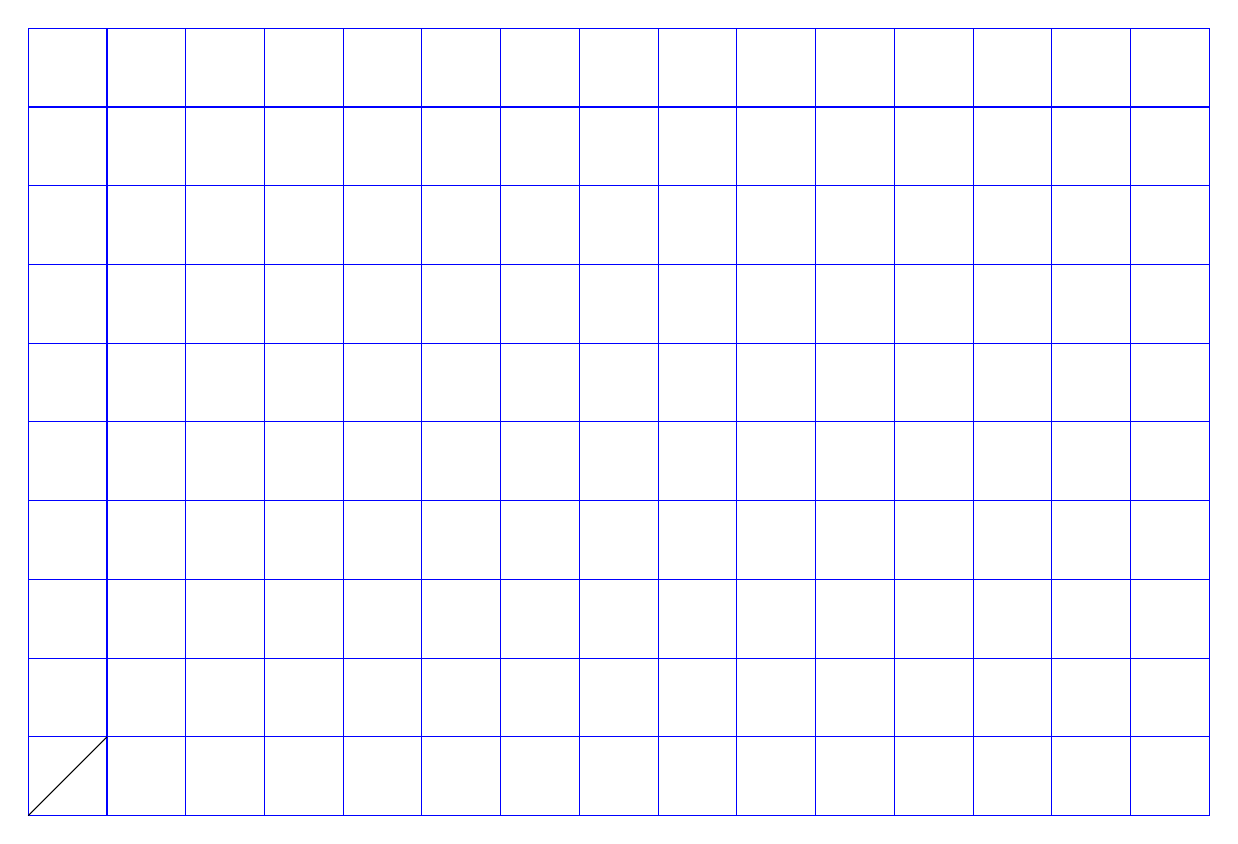
\begin{tikzpicture}
\draw[step=1cm,blue,thin] (0,0) grid (15,10);
\draw (0,0) -- (1,1);
\end{tikzpicture}

\blindtext

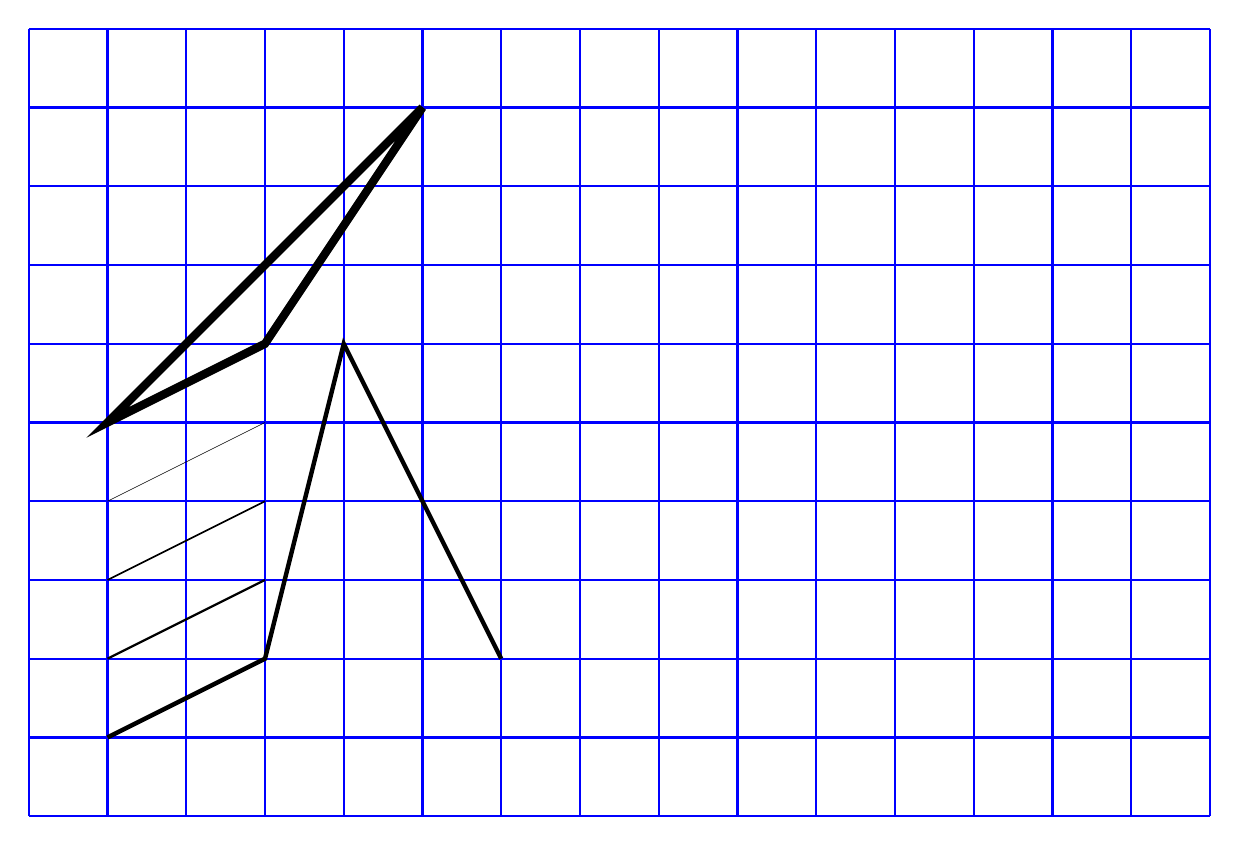
\begin{tikzpicture}
\draw[step=1cm,blue,thick] (0,0) grid (15,10);
\draw[ultra thick] (1,1) -- (3,2) -- (4,6) -- (6,2);
\draw[thick] (1,2) -- (3,3);
\draw[semithick] (1,3) -- (3,4);
\draw[very thin] (1,4) -- (3,5);
\draw[line width=3pt] (1,5) -- (3,6) -- (5,9) -- cycle; % schließt Polygonzug
\end{tikzpicture}

\blindtext

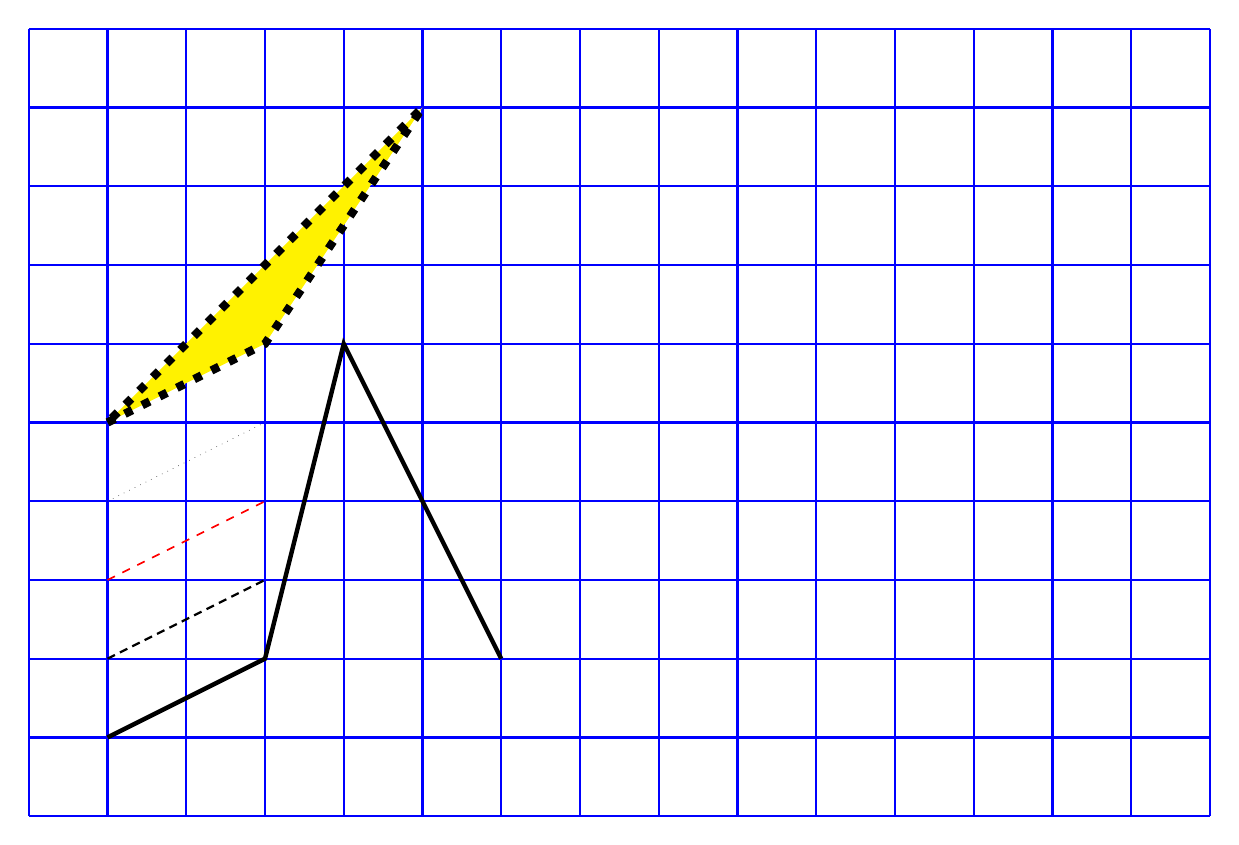
\begin{tikzpicture}
\draw[step=1cm,blue,thick] (0,0) grid (15,10);
\draw[ultra thick] (1,1) -- (3,2) -- (4,6) -- (6,2);
\draw[thick, densely dashed] (1,2) -- (3,3);
\draw[semithick, dashed,red] (1,3) -- (3,4);
\draw[very thin,dotted] (1,4) -- (3,5);
\draw[line width=3pt, loosely dotted,fill=yellow] (1,5) -- (3,6) -- (5,9) -- cycle; % schließt Polygonzug
\end{tikzpicture}


\blindtext

Relative Koordinaten: ausgehend von Punkt 1,1 gehe 5 Einheiten nach rechts und eine hoch!

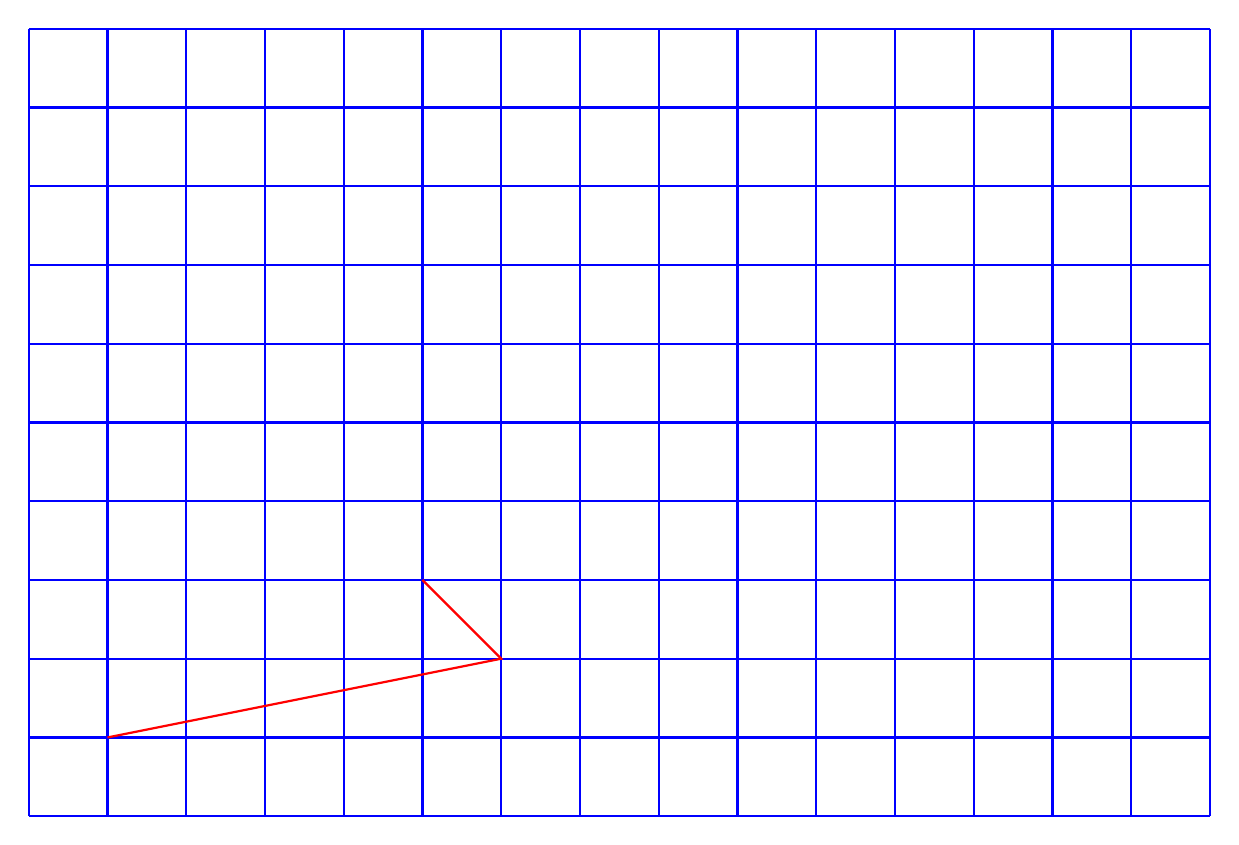
\begin{tikzpicture}
\draw[step=1cm,blue,thick] (0,0) grid (15,10);
\draw[thick,red] (1,1) -- ++ (5,1) -- ++ (-1,1) ;
\end{tikzpicture}


\section{Relative Koordinaten ohne Update!}

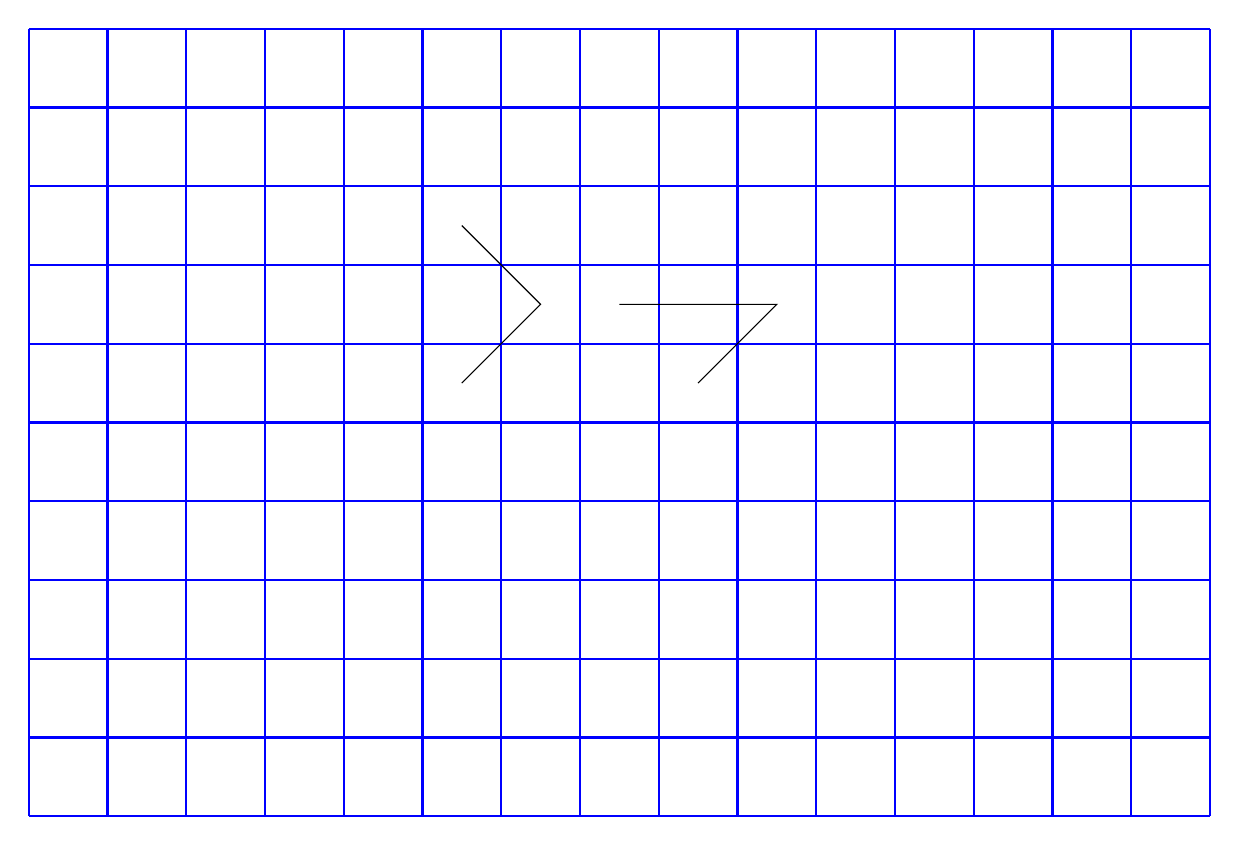
\begin{tikzpicture}
\draw[step=1cm,blue,thick] (0,0) grid (15,10);
% ++-Version nimmt den letzten Punkt als Ausgangsbasis
\draw (5.5,5.5) -- ++(1,1) -- ++(-1,1);

% +-Version nimmt immer den ersten Punkt als Ausgangsbasis
\draw (8.5,5.5) -- +(1,1) -- +(-1,1);
\end{tikzpicture}

\section{Polarkoordinaten}


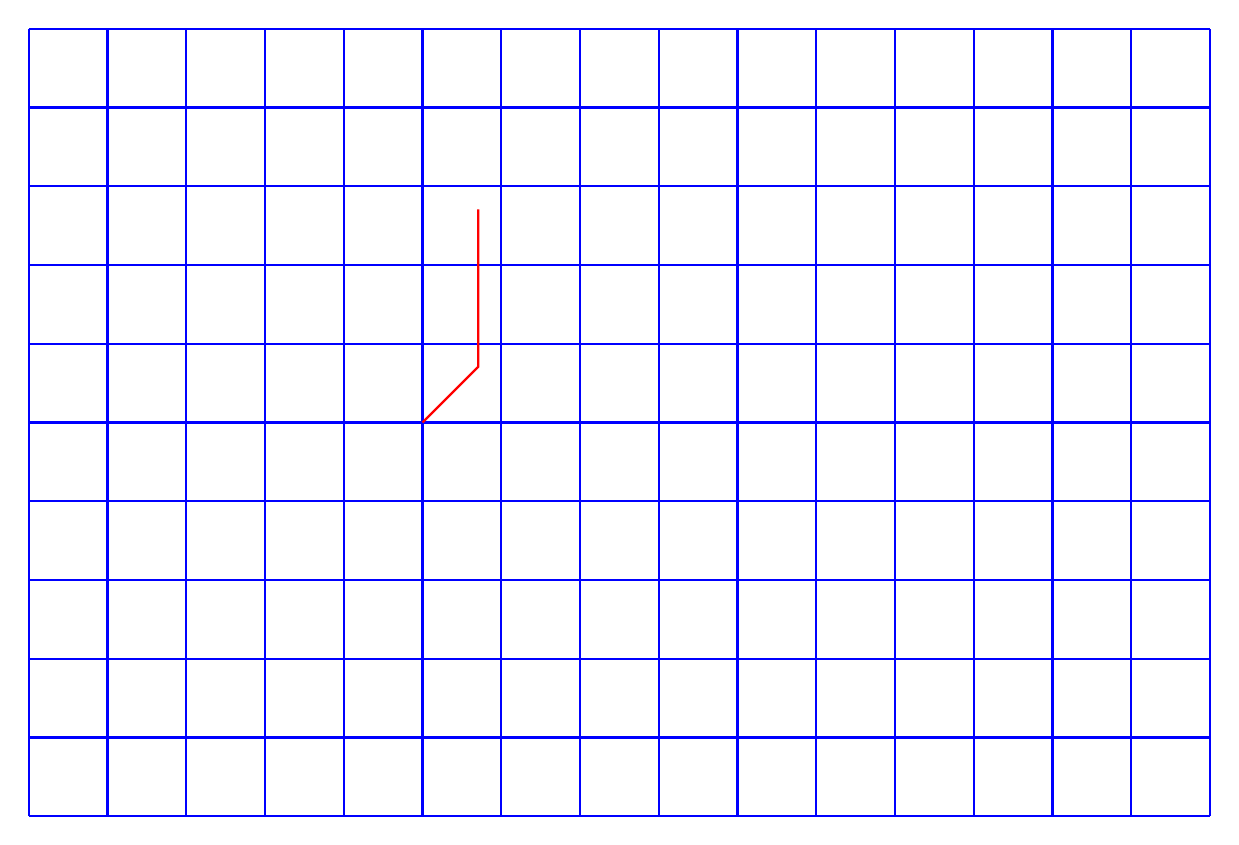
\begin{tikzpicture}
\draw[step=1cm,blue,thick] (0,0) grid (15,10);
\draw[thick,red] (5,5) -- ++ (45:1) -- ++ (90:2);
\end{tikzpicture}

\section{Nodes und Coordinates}

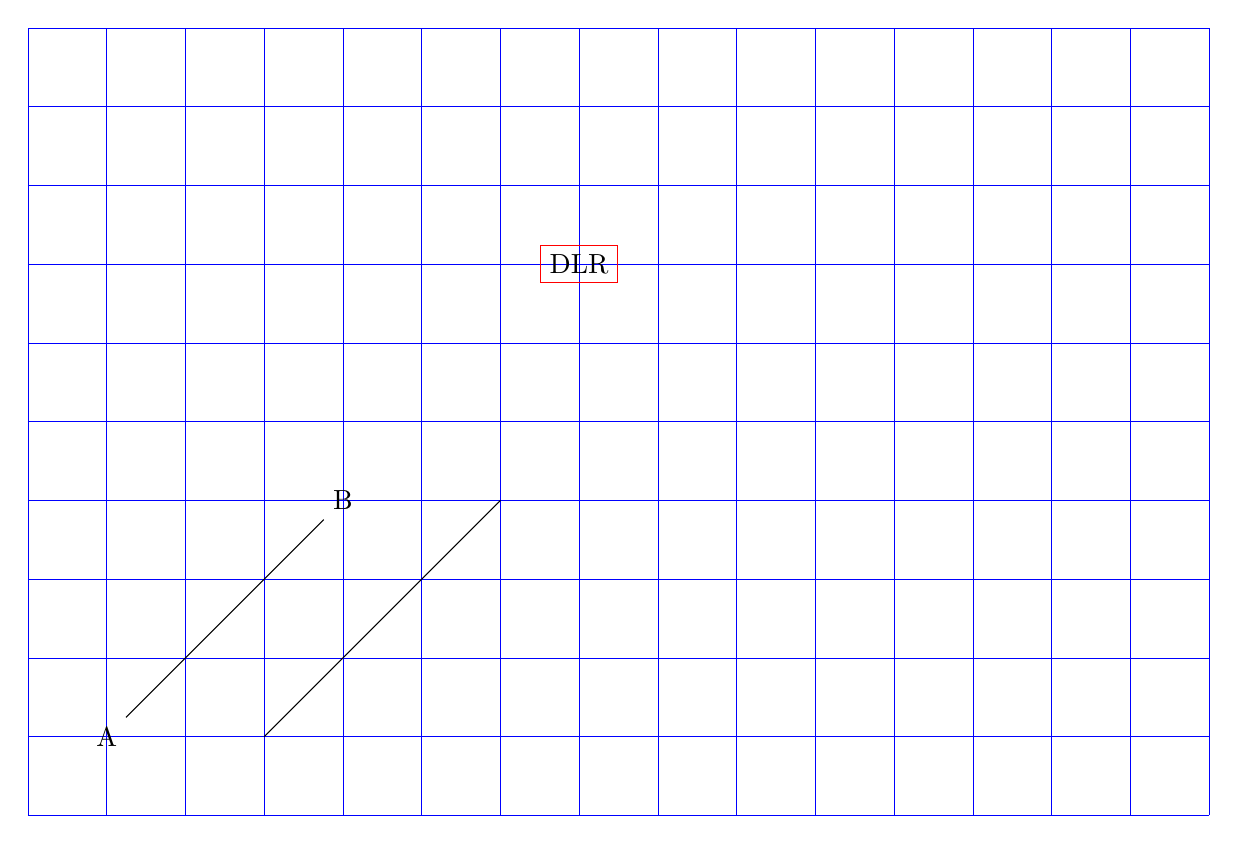
\begin{tikzpicture}
\draw[step=1cm,blue,very thin] (0,0) grid (15,10);

\node (a) at (1,1){A}; % Label muss angegeben werden, kann leer sein
\node (b) at (4,4){B};
\draw (a) -- (b);

\coordinate (c) at (3,1); 
\coordinate (d) at (6,4);
\draw (c) -- (d);

\node[rectangle,draw=red] (e) at (7,7){DLR};

\end{tikzpicture}

\end{document}